\chapter{Kalman Filter} \labchap{kalman_filter}

\section{Introduction} 
The Kalman Filter is a recursive algorithm introduced in the 1960's as a method to track, estimate, and predict the state of a system and corresponding uncertainties \cite{Kalman:1960}.
This filter integrates a dynamic (linear) model of the system, control inputs, measurements, and biases/uncertainties into a single algorithm.
This effectively fuses together system inputs and responses and extrapolates what the system is currently doing and expected to do.
One key advantage of this algorithm is that it only requires the guess of the previous state to estimate the current state. 
This massively decreases the memory and processing costs as the history of inputs, measurements, and uncertainties does not need to be remembered or analyzed.
However, it does have some limitations when the sensor data is noisy or the control inputs cannot be linearly mapped to the system state.
Random errors in the sensor data may cause the filter to behave unpredictably and non-linearity prevents proper fusion entirely.
This problem can be solved using an Extended Kalman Filter, but that is out of scope for now.

\section{Kalman Filter in One Dimension}
The uni-dimensional Kalman filter is a special, idealized case for the Kalman filter.
It is more convenient as a teaching tool as it does not include the complex matrix and vector operations the general multi-dimensional Kalman filter requires.
However, this only makes this type useful for tracking and estimating a single variable.

Multiple uni-dimensional Kalman filters can be run in parallel or chained together to mimic a multi-dimensional filter, however, this will unnecessarily increase the computational resources required for the calculations and will reduce the quality of the filtering overall.

\subsection{The Kalman Gain} 
In a Kalman filter, the Kalman Gain, denoted as $K_n$, is calculated at each iteration of the filter.
The Kalman gain is bounded by: $0 <= Kn <= 1$ and prioritizes predictions of the system state from the estimation or the measurement, based on related uncertainties\footnote{\textbf{Important note:} When measurement uncertainty is very large, and the estimate uncertainty is small, $K_n << 1$, hence big weight to the estimate and small weight to the measurement. When the opposite is true, $K_n -> 1$, meaning a large weight to the measurement and a small weight to the estimate. This is how the Kalman filter can regulate and smooth out noisy data by knowing the uncertainties.}.

\begin{equation} \labeq{kalman_gain}
    \begin{aligned}
        K_n &= \frac{\text{Estimate Uncertainty}}{\text{Estimate Uncertainty + Measurement Uncertainty}} \\
            &= \frac{p_{n,n-1}}{p_{n,n-1} + r_n}
    \end{aligned}
\end{equation}

We can then define the State Update Equation for a system where $\hat{x}$ is the predicted state and $z$ is the measured state:

\begin{equation} \labeq{kalman_state_update}
    \begin{aligned}
        \hat{x}_{n,n} &= \hat{x}_{n,n-1} + K_n(z_n - \hat{x}_{n,n-1}) \\
                        &= (1-K_n)\hat{x}_{n,n-1} + K_n z_n \\
    \end{aligned}
\end{equation}

\subsection{The Estimate Uncertainty Update Equation} 
The estimate uncertainty or covariance update equation predicts the uncertainty associated with the current estimate.
The estimate uncertainty should approach (converge) to 0 with each filter iteration as the filter improves its guessing accuracy.
However, if the measurement uncertainty is large ($K_n << 1$), the estimate uncertainty will converge more slowly.
The opposite is true if the measurement uncertainty is small.
Basically, the more precise your measurements are, the faster the Kalman filter will converge on the best estimate.

\begin{gather}
    p_{n,n} = (1-K_n)p_{n,n-1} \\
    \begin{aligned}
        \text{where } &p_{n,n} \text{ is the estimate uncertainty at the current state} \\
                        &K_n \text{ is the Kalman gain at the current state} \\
                        &p_{n,n-1} \text{ is the estimate uncertainty of the previous state}
    \end{aligned} \notag
\end{gather}

\subsection{The Estimate Uncertainty Extrapolation Equation} 
Another Kalman equation is how the filter predicts future uncertainties and is called the Estimate Uncertainty Extrapolation Equation or the Estimate Covariance Extrapolation Equation.
Like with the State Extrapolation Equations, this is done with dynamic models and will be unique to every example.
FOr a moving vehicle, one example might be:

\begin{gather} \labeq{covariance_extrapolation}
    p_{n+1,n}^x = p_{n,n}^x + \Delta t p_{n,n}^{\dot{x}} \\
    p_{n+1,n}^{\dot{x}} = p_{n,n}^{\dot{x}} \\
    \begin{aligned}
    \text{where } &x \text{ is the vehicle displacement, and} \\
                  &\dot{x} \text{ is the vehicle velocity}
    \end{aligned}
\end{gather}

\subsection{Putting it all Together}
First, the filter is initialized with a first guess ($\hat{x}_{0,0}$) and an associated uncertainty ($p_{0,0}$).
These values are passed into the dynamic model equations and Equation \ref{eq:covariance_extrapolation} to predict the state at the first measurement ($x_{1,0}$) and the associated uncertainty ($p_{1,0}$).
This is shown as Step 0 in Figure \ref{fig:kalman_filter_process}.
Then, we can take a measurement ($z_n$) and record its uncertainty ($r_n$), using the latter to determine the Kalman gain with Equation \ref{eq:kalman_gain}.
We can then estimate the current state value using Equation \ref{eq:kalman_state_update} using the recorded measurement and the Kalman gain ($K_n$).
The current state estimate and its uncertainty can then be outputted from the filter and used in applications; this process is shown as Steps 1, 2a, and 2b in the figure below.
These values are then fed into the dynamic model to predict the next state and estimate the associated uncertainty (Step 3 in the below diagram).
Optionally, these predicted values can be outputted from the model as well, as the application requires.
This process repeats for every measurement with $n$ incrementing every time.

\begin{figure}[h!]
    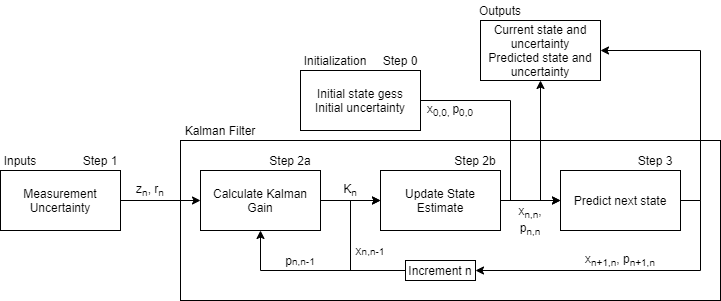
\includegraphics[width=\textwidth]{appendices/kalman-filter/KalmanFilter.png}
    \caption[Kalman Filter Diagram]{Process diagram for a Kalman filter.}
    \labfig{kalman_filter_process}
\end{figure}

\begin{fitbox}[frametitle=Example]
    In this example, we will be estimating the depth of an ROV using a 1D Kalman filter.
    We will be assuming the ROV depth remains constant and its location in space does not matter or change.
    For example's sake, we shall know for an absolute fact that the ROV is at a depth of 50-meters ($x=50 \text{ m}$).
    We will also assume that our depth sensor has a standard deviation of 5-meters ($\sigma=5 \text{ m}$), therefore we will have a measurement variance or uncertainty of 25-meters ($r=25 \text{ m}^2$)

    \paragraph*{Iteration 0}
    \begin{equation*}
        \begin{aligned}
            0 &: \text{Estimate depth: } \hat{x}_{0,0} = \textbf{60 m} \\
                &: \text{Estimate uncertainty: } p_{0,0} = \textbf{225 m}^2 \\
            3 &: \text{Predicted depth: } \hat{x}_{1,0} = \hat{x}_{0,0} = \textbf{60 m} \\
                &: \text{Prediction uncertainty: } p_{1,0} = p_{0,0} = \textbf{225 m}^2 \\
        \end{aligned}
    \end{equation*}

    \paragraph*{Iteration 1}
    \begin{equation*}
        \begin{aligned}
            1 &: \text{Measure depth: } z_1 = \textbf{48.54 m} \\
                &: \text{Measurement uncertainty: } r_1 = \textbf{25 m}^2 \\
            2 &: \text{Kalman gain } K_1 = \frac{p_{1,0}}{p_{1,0}+r_1} = \frac{255}{255 + 25} = \textbf{0.9} \\
                &: \text{Estimated depth: } \hat{x}_{1,1} = \hat{x}_{1,0} + K_1(z_1 - \hat{x}_{1,0}) = 60 + 0.9(48.54-60) = \textbf{49.69 m} \\
                &: \text{Estimate uncertainty: } p_{1,1} = (1-K_1)p_{1,0} = (1-0.9)225 = \textbf{22.5 m}^2 \\
            3 &: \text{Predicted depth: } \hat{x}_{2,1} = \hat{x}_{1,1} = \textbf{49.69 m} \\
                &: \text{Prediction uncertainty: } p_{1,0} = p_{1,1} = \textbf{22.5 m}^2 \\
        \end{aligned}
    \end{equation*}

    \paragraph*{Iteration 2}
    \begin{equation*}
        \begin{aligned}
            1 &: \text{Measure depth: } z_2 = \textbf{47.11 m} \\
                &: \text{Measurement uncertainty: } r_2 = \textbf{25 m}^2 \\
            2 &: \text{Kalman gain } K_2 = \frac{p_{2,1}}{p_{2,1}+r_2} = \frac{22.5}{22.5 + 25} = \textbf{0.47} \\
                &: \text{Estimated depth: } \hat{x}_{2,2} = \hat{x}_{2,1} + K_2(z_2 - \hat{x}_{2,1}) = 49.69 + 0.47(47.11-49.69) = \textbf{48.47 m} \\
                &: \text{Estimate uncertainty: } p_{2,2} = (1-K_2)p_{2,1} = (1-0.47)22.5 = \textbf{11.84 m}^2 \\
            3 &: \text{Predicted depth: } \hat{x}_{3,2} = \hat{x}_{2,2} = \textbf{48.47 m} \\
                &: \text{Prediction uncertainty: } p_{3,2} = p_{2,2} = \textbf{11.84 m}^2 \\
        \end{aligned}
    \end{equation*}

    \begin{center}
        \begin{tabular}{c | c | c | c | c | c | c | c}
        \toprule
        & \multicolumn{2}{c}{Measurements} & \multicolumn{3}{c}{Current Estimates} & \multicolumn{2}{c}{Predictions} \\
        \midrule
        n & $z_n$ & $r_n$ & $K_n$ & $\hat{x}_{n,n}$ & $ p_{n,n} $ & $ \hat{x}_{n+1,n}$ & $ p_{n+1,n} $ \\
        \midrule

        0  & ---  & -- & ---  & 60.0 & 225  & 60.0 & 225  \\
        1  & 48.5 & 25 & 0.90 & 49.7 & 22.5 & 49.7 & 22.5 \\
        2  & 47.1 & 25 & 0.47 & 48.4 & 11.8 & 48.4 & 11.8 \\
        3  & 55.0 & 25 & 0.32 & 50.6 & 8.03 & 50.6 & 8.03 \\
        4  & 55.2 & 25 & 0.24 & 51.7 & 6.08 & 51.7 & 6.08 \\
        5  & 49.9 & 25 & 0.20 & 51.3 & 4.89 & 51.3 & 4.89 \\
        6  & 40.6 & 25 & 0.16 & 49.6 & 4.09 & 49.6 & 4.09 \\
        7  & 46.7 & 25 & 0.14 & 49.2 & 3.52 & 49.2 & 3.52 \\
        8  & 50.1 & 25 & 0.12 & 49.3 & 3.08 & 49.3 & 3.08 \\
        9  & 51.3 & 25 & 0.11 & 49.5 & 2.74 & 49.5 & 2.74 \\
        10 & 50.0 & 25 & 0.10 & 49.6 & 2.47 & 49.6 & 2.47 \\

        \bottomrule
        \end{tabular}
    \end{center}

    \begin{center}
        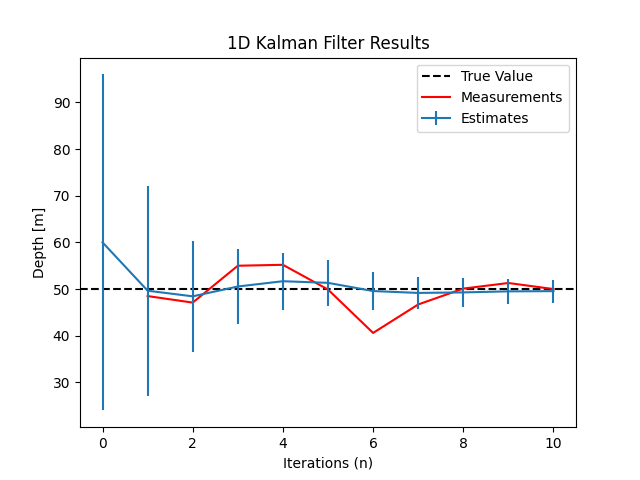
\includegraphics[height=3in]{appendices/kalman-filter/1D_kalman_filter_results.png}
    \end{center}

    We can see from the figure that the Kalman filter eventually converges on the true value and considerably smoothes out the noisy measurements.
    The error bars on the estimate plot (blue) also show that the Kalman filter increases its confidence with every iteration as it converges to the true value.
    The oscillation shown in the estimates are a result of the gains being slightly off from their ideal value.
    Tuning the process noise variable (q) can cause the filter to converge quickly and confidently to the true value in fewer iterations.

\end{fitbox}

\subsection{Process Noise} In the real world, there are uncertainties in the system's dynamic model.
Uncertainty is caused by unanticipated changes in the system due to external factors.
This can be drift caused by ocean current, wind blowing a rocket to the side, drag, friction, even time dilation in extreme cases.
Generally, these uncertainties can be combined into the Process Noise gain denoted by $q$.
To account for process noise, it must be included in the Covariance Extrapolation Equation (Equation \ref{eq:covariance_extrapolation}).

If the model is not known to be good or is very noisy, we can increase the process noise gain to reduce the lag error.

\begin{equation}
    p_{n+1,n} = p_{n,n} + q
\end{equation}

\subsection*{Further Reading}
The book \textit{Kalman Filter: From the Ground Up} \cite{Becker:2023} provides an excellent resource on the intuitive understanding of the Kalman Filter and some of its more advanced applications like multi-variate Kalman Filters, Extended Kalman Filters, and applying Kalman Filters in sensor fusion applications.